\documentclass[dvipdfmx]{beamer}
\usetheme[
    block=fill, % ブロックに背景をつける
    progressbar=foot, % 各スライドの下にプログレスバー
    numbering=fraction % 合計ページ数を表示
]{metropolis}         % Use metropolis theme
\usepackage{float}
\usepackage{listings,jvlisting} %日本語のコメントアウトをする場合jvlisting(もしくはjlisting)が必要
%ここからソースコードの表示に関する設定
\lstset{
  basicstyle={\ttfamily},
  identifierstyle={\small},
  commentstyle={\smallitshape},
  keywordstyle={\small\bfseries},
  ndkeywordstyle={\small},
  stringstyle={\small\ttfamily},
  frame={tb},
  breaklines=true,
  columns=[l]{fullflexible},
  numbers=left,
  xrightmargin=0zw,
  xleftmargin=3zw,
  numberstyle={\scriptsize},
  stepnumber=1,
  numbersep=1zw,
  lineskip=-0.5ex
}

\title{Progress}
\date{\today}
\author{Mizuno Yasuaki}
%\institute{Centre for Modern Beamer Themes}
\begin{document}
  \maketitle
  
  \begin{frame}{目次}
    \begin{itemize}
      \item アミノ酸ベクタの割り当て①
      \item 学習結果①
      \item アミノ酸ベクタの割り当て②
      \item 学習結果②
      \item まとめ
    \end{itemize}
  \end{frame}

  \begin{frame}{アミノ酸ベクタの割り当て①}
    x成分をアミノ酸のサイズ、y成分を疎水性尺度とした。
    \begin{table}[H]
      \centering
      \caption{アミノ酸ベクタ}
      \label{tab:amino_vector_1}
      \begin{tabular}{cccc}
        \hline
        アミノ酸 & (x, y) & アミノ酸 & (x, y) \\
        \hline \hline
        A & (2.5, 0.02) & M & (6.0, 1.00) \\
        C & (3.0, 0.77) & N & (5.0, -0.77) \\
        E & (5.0, -1.14) & P & (5.5, -0.09) \\
        F & (2.5, 1.35) & Q & (6.0, -1.10) \\
        G & (0.5, -0.80) & S & (3.0 -0.97) \\
        H & (6.0, 0.26) & T & (5.0, 1.13) \\
        I & (5.5, 1.81) & V & (5.0, 1.13) \\
        K & (7.0, -0.41) & W & (7.0, 1.71) \\
        L & (5.5, 1.14) & Y & (7.0, 1.11) \\
        \hline
      \end{tabular}
    \end{table}
  \end{frame}

  \begin{frame}
    \begin{figure}
      \centering
      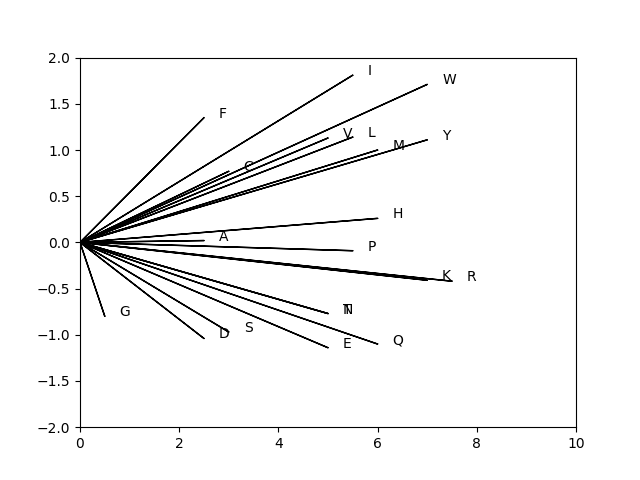
\includegraphics[keepaspectratio, scale=0.6]{images/amino_vector.png}
      \caption{アミノ酸ベクタ①}
    \end{figure}
  \end{frame}

  \begin{frame}{モデル①}
    \begin{block}{モデル①}
      \begin{itemize}
        \item 全結合層
        \begin{itemize}
          \item 活性化関数 \mbox{} Relu
          \item Heの初期値
          \item l2正規化
        \end{itemize}
        \item adam(learning\_rate=0.001)
        \item batch\_size = 128
        \item epochs = 20
      \end{itemize}
    \end{block}
  \end{frame}

  \begin{frame}
    Test accuracy: 0.9567307829856873
    \begin{figure}
      \centering
      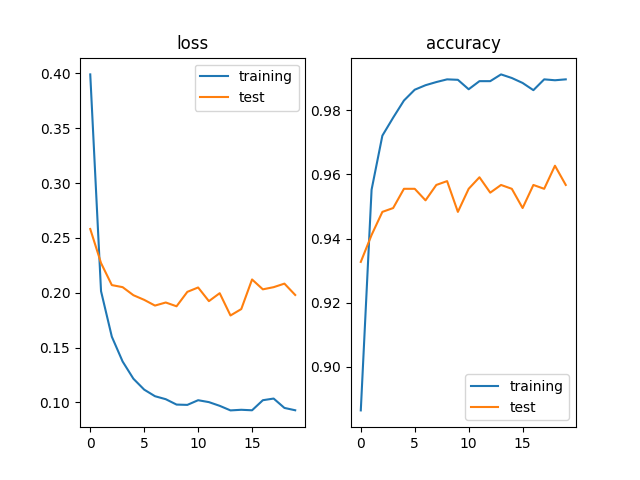
\includegraphics[keepaspectratio, scale=0.6]{images/train_ffn.png}
      \caption{モデル①の学習結果①}
    \end{figure}
  \end{frame}

  \begin{frame}
    Test accuracy: 0.9543269276618958
    \begin{figure}
      \centering
      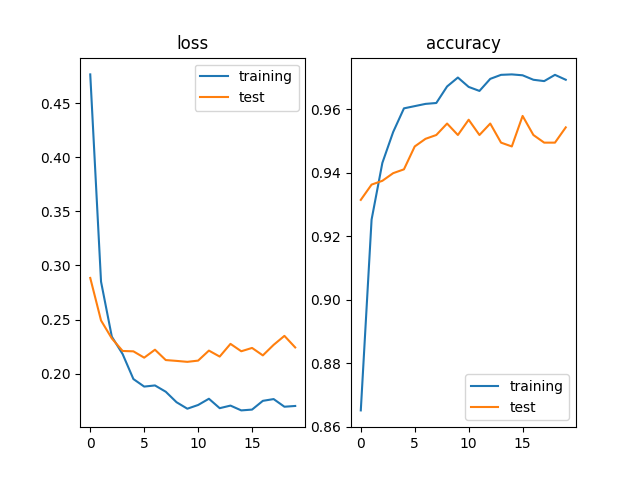
\includegraphics[keepaspectratio, scale=0.6]{images/train_ffn_dropout.png}
      \caption{モデル①の学習結果}
    \end{figure}
  \end{frame}

  \begin{frame}{モデル①の学習結果①}
    \begin{table}[H]
      \centering
      \caption{各クラスにおける正解率}
      \begin{tabular}{cr}
        \hline
        class & accuracy \\
        \hline \hline
        A & 0.9718309640884399 \\
        B & 0.7884615659713745 \\
        C & 0.9567307829856873 \\
        D & 0.0 \\
        E & 1.0 \\
        \hline
      \end{tabular}
    \end{table}
  \end{frame}

  \begin{frame}{アミノ酸ベクタの割り当て②}
    \begin{table}[h]
      \caption{アミノ酸の疎水性度}
      \begin{tabular}{cccc}
          \hline
          アミノ酸 & 疎水性度 & アミノ酸 & 疎水性度 \\
          \hline \hline 
          Arg/R & -5.10 & Gly/G & -0.64 \\
          Lys/K & -4.11 & Ser/S & -0.50 \\
          Gln/Q & -3.68 & Trp/W & -0.46 \\
          Asp/D & -3.60 & Ala/A & 1.10 \\
          Asn/N & -3.50 & Met/M & 1.90 \\
          His/H & -3.20 & Cys/C & 2.50 \\
          Glu/E & -3.20 & Phe/F & 2.80 \\
          Pro/P & -1.90 & Leu/L & 3.80 \\
          Tyr/Y & -1.30 & Val/V & 4.20 \\
          Thr/T & 0.70 & Ile/I & 4.50 \\
          \hline
      \end{tabular}
    \end{table}
  \end{frame}

  \begin{frame}{アミノ酸ベクタの割り当て②}
    疎水精度をhとする。任意のアミノ酸 \(c\) におけるベクトルを以下に示す。
    \[
      \left\{ \,
          \begin{aligned}
          & \theta = 180 - 170 \times \frac{h_c + |h_{min}|}{|h_{max}| + |h_{min}|} \\
          & x = cos{\theta} \\
          & y = sin{\theta}
          \end{aligned}
      \right.
    \]   
  \end{frame}

  \begin{frame}
    \begin{figure}
      \centering
      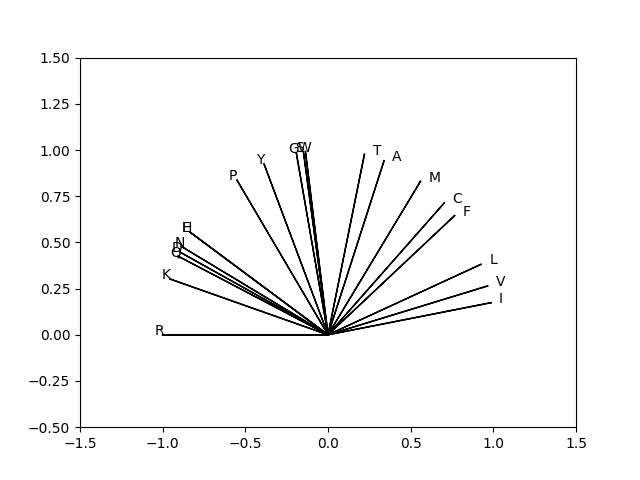
\includegraphics[keepaspectratio, scale=0.6]{images/my_amino_vector.png}
      \caption{アミノ酸ベクタ②}
    \end{figure}
  \end{frame}

  \begin{frame}
    Test accuracy: 0.9435096383094788
    \begin{figure}
      \centering
      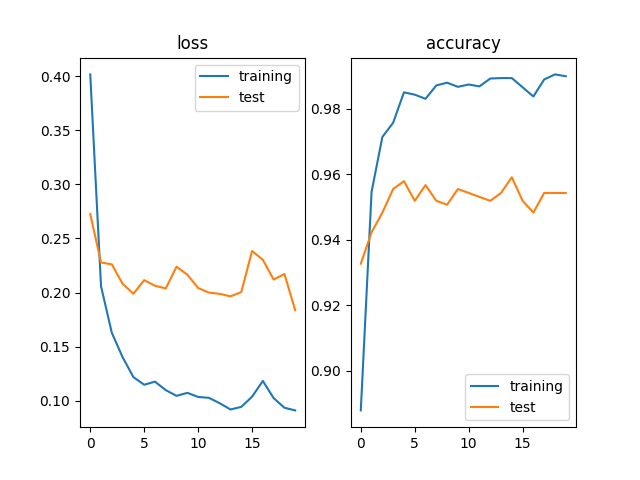
\includegraphics[keepaspectratio, scale=0.6]{images/train_my_ffn.png}
      \caption{モデル①の学習結果②}
    \end{figure}
  \end{frame}

  \begin{frame}
    Test accuracy: 0.9543269276618958
    \begin{figure}
      \centering
      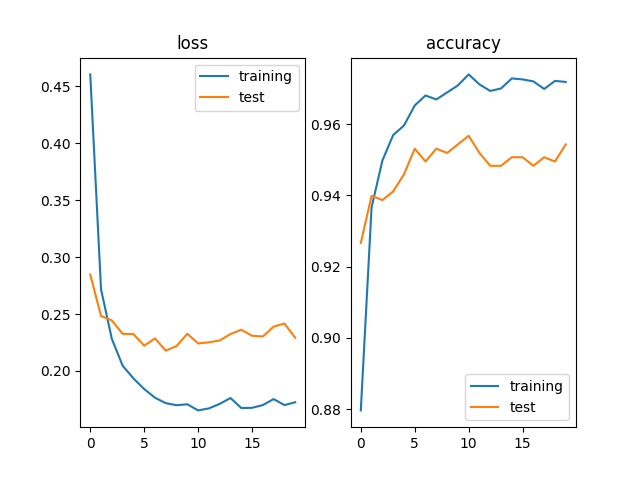
\includegraphics[keepaspectratio, scale=0.6]{images/train_my_ffn_dropout.png}
      \caption{モデル①の学習結果②}
    \end{figure}
  \end{frame}

  \begin{frame}{モデル①の学習結果②}
    \begin{table}[H]
      \centering
      \caption{各クラスにおける正解率}
      \begin{tabular}{cr}
        \hline
        class & accuracy \\
        \hline \hline
        A & 0.966549277305603 \\
        B & 0.807692289352417 \\
        C & 0.961538434028625 \\
        D & 0.0 \\
        E & 1.0 \\
        \hline
      \end{tabular}
    \end{table}
  \end{frame}

  \begin{frame}{まとめ}
    \begin{itemize}
      \item クラスDとクラスEの正答率が小さかった
      \item 単純なニューラルネットワークを試したので、より複雑なニューラルネットワークを使う
      \item COGのデータベースで試す
    \end{itemize}
  \end{frame}

\end{document}


